\documentclass[a4paper]{standalone}
\usepackage{amsmath}
\usepackage{circuitikz}
\usetikzlibrary{fit, shapes, arrows, patterns, decorations.text, decorations.markings}

\begin{document}
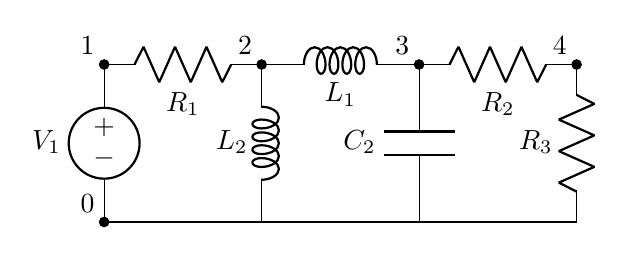
\begin{tikzpicture}[scale=1.00, transform shape, /tikz/circuitikz/bipoles/length=1.50cm, american currents, american voltages, voltage dir=RP]
  \coordinate (1) at (0,2);
  \coordinate (0) at (0,0);
  \coordinate (2) at (2,2);
  \coordinate (3) at (4,2);
  \coordinate (4) at (6,2);
  \coordinate (0_2) at (2,0);
  \coordinate (0_3) at (4,0);
  \coordinate (0_4) at (6,0);
  \draw (0) to [V, l^=$V_{1}$, n=V1] (1);
  \draw (1) to [R, l_=$R_{1}$, n=R1] (2);
  \draw (2) to [L, l_=$L_{1}$, n=L1] (3);
  \draw (3) to [R, l_=$R_{2}$, n=R2] (4);
  \draw (2) to [L, l_=$L_{2}$, n=L2] (0_2);
  \draw (3) to [C, l_=$C_{2}$, n=C2] (0_3);
  \draw (4) to [R, l_=$R_{3}$, n=R3] (0_4);
  \draw[-] (0) to (0_2);
  \draw[-] (0_2) to (0_3);
  \draw[-] (0_3) to (0_4);
  \draw (1) node[circ] {};
  \draw (0) node[circ] {};
  \draw (2) node[circ] {};
  \draw (3) node[circ] {};
  \draw (4) node[circ] {};
  \draw[anchor=south east] (1) node {1};
  \draw[anchor=south east] (0) node {0};
  \draw[anchor=south east] (2) node {2};
  \draw[anchor=south east] (3) node {3};
  \draw[anchor=south east] (4) node {4};
\end{tikzpicture}
\end{document}